\chapter{Translating source code}
\label{chap:TranslatingCode}
\mtoc

In this chapter, we describe our solution which is based on generating and evaluating method names by translating the source code of a method into English. We first talk explain why it makes sense to think of our problem in terms of machine translation, then we describe our solution in all details, including how we prepared the dataset for training, what model did we use and how we tuned its parameters.

% At the end of this chapter we do a quick overview of the generated names and visualize the attention of our model to better understand which tokens contribute the most to the selection of each name.

\section{Reasoning behind translating code}
\label{sec:TranslatingCode-Reasoning}

As we have seen in Chapter \ref{chap:Naturalness}, the source code has statistical properties similar to natural languages that allow us to build predictive models on source code similarly to how we do it in natural language processing.

Translating source code from one programming language into another is not a trivial task and it can not be done with end-to-end deep learning approaches, as we do it with natural languages. This is explained by the differences between code and natural text. Code is formal and executable. Changing order of words in a sentence, or incorrectly translating one word can reduce the quality of the translation, but we will still be able to understand the overall meaning of a sentence. This is different in source code - consider swapping two arguments of a function, or choosing a wrong token - such code will most likely be non-executable or produce wrong results. Therefore, when translating code between programming languages, we must combine our probabilistic language models with complex heuristics that will preserve the executability of results.

In our work, however, we consider a different problem. We translate source code of Smalltalk into very short English sentences, a couple of words that describe what a given piece of code is doing and can be concatenated into a method name. Even though Smalltalk, the source language of our translation, is formal and executable, English, the target language, is natural. This means that the noisy results produced by our model will be just as useful as the result of English-French translation.

\section{Formal problem statement}
\label{sec:TranslatingCode-Problem}

We are given a set of methods represented by pairs

\[ P = \{(x^{(i)}, y^{(i)}) | i = 1, \dots N \} \]

where

\[ x^{(i)} = x_1^{(i)}, x_2^{(i)}, \dots, x_{n_i}^{(i)},\ x_k^{(i)} \in V_x \]

is a method body tokenized into a sequence of source tokens and

\[ y^{(i)} = y_1^{(i)}, y_2^{(i)}, \dots, y_{m_i}^{(i)},\ y_k^{(i)} \in V_y \]

is a sequence of English words that can be concatenated with camel-case into a method name. For example,

\begin{align*}
  x^{(i)} &= \text{\textit{"self", "assert", ":", "<num>", "+", "<num>", "equals", ":", "<num>", "."}}\\
  y^{(i)} &= \text{\textit{"test", "add"}}
\end{align*}

$|x^{(i)}| = n_i$ is the length of the input sequence, number of tokens in the source code of a method, and $|y^{(i)}| = m_i$ is the length of the output sequence, number of words in the method name. Both sequences can have various length, it is possible that for $i \neq j$, $n_i \neq n_j$, $m_i \neq m_j$, or $n_i \neq m_i$.

We need to find a function $f$ which maps $x$ to $y$ by assigning a sequence $h^{(i)} = h_1^{(i)}, h_2^{(i)}, \dots, h_{p_i}^{(i)},\ h_k^{(i)} \in V_y$ for every input sequence $x^{(i)}$ in such way that it minimizes the negative log-likelihood\footnote{In Section \ref{sec:Background-Likelihood} of the Appendix we explain why cross-entropy is called negative log-likelihood and why do we train machine learning models by minimizing it.} (cross-entropy) between $y^{(i)}$ and $h^{(i)}$.

\section{Data preparation}
\label{sec:TranslatingCode-Data}

In this section, we discuss in details how we filtered and preprocessed the dataset of Pharo methods to prepare it for our model (we have explained how this data was collected in Section \ref{tab:Naturalness-DataPharo}). This is a very important part of our solution because we have noticed that the selection of good training examples and their correct representation has a more significant impact on the performance than the good choice of model and values of hyperparameters.

\subsubsection{Duplicated methods}
\label{sec:TranslatingCode-Duplicate}

Some methods are highly repetitive across different classes, which means that some source-name pairs will be better represented in the dataset, which makes it harder to interpret how the model is learning (did it learn to map semantics of source code to method names, or does it simply memorize highly repetitive patterns?). It is also crucial that the replicas of the same method do not appear in both training and test sets (discussed in more details in Section \ref{sec:TranslatingCode-TrainValidTest}). For that reason, we have removed all duplicates from our dataset.

\subsubsection{Non-informative methods}

We have removed all abstract methods since their bodies consist of a single line \lstinline{self subclassResponsibility} which does not provide enough information to suggest a name. We also removed instance side methods that return the receiver \lstinline{^ self} because the name suggestions for these methods can only be based on class names, not the source code. We didn't remove methods that return constant values such as numbers, string literals, and points \lstinline{400@500} because the model can learn to assign them with names such as \lstinline{defaultSize}, \lstinline{title}, \lstinline{extent} etc.

\subsubsection{Overriden methods}

\cite{Alla16} also remove the overridden methods based on the claim that they are highly repetitive and easy to predict. However, we keep these methods because their implementations are different and it is not trivial for a machine learning model to notice the similarity between two implementations of the same method and label them with the same name. And in the end, that is exacly what we want our model to learn.

\begin{lstlisting}
Dictionary >> collect: aBlock
  | newCollection |
  newCollection := self species new.
  self associationsDo:[:each |
    newCollection at: each key put: (aBlock value: each value).
  ].
  ^newCollection

LinkedList >> collect: aBlock
  | aLink newCollection |
  newCollection := self class new.
  aLink := firstLink.
  [aLink == nil] whileFalse:
    [newCollection add: (aBlock value: aLink value).
    aLink := aLink nextLink].
  ^ newCollection
\end{lstlisting}

\subsection{Tokenizing source code}
\label{sec:TranslatingCode-TokenizingSource}

Unlike natural languages, executable source code can always be non-ambiguously divided into tokens. However, the process of tokenizing source code is much harder than that on English. Even though English may have ambiguous compound words (\textit{ice box = ice-box = icebox}), in general we can separate words by spaces and punctuation: \textit{"Mrs. Smith is sleeping"} $\rightarrow$ \textit{"mrs", "smith", "is", "sleeping"}. This can not be easily done with most programming languages because

\begin{enumerate}
  \item In many languages (Java, C) spaces are optional and in languages like Pharo, where spaces separate receivers and messages, they are still optional about operators \lstinline{+, -, *, /, =, >} etc. and brackets \lstinline|(), [], {}|.
  \item In programming languages, both string literals and comments are treated as a single token, however, they can have multiple spaces inside.
\end{enumerate}

Therefore, tokenization of source code such as the line in the following example can not be done by simply splitting the code by space. It requires a complex parser which has the full knowledge of a syntax of the given language.

\begin{lstlisting}[language=Java]
student.name=form.getValue("First name");
\end{lstlisting}

Pharo is almost entirely written in itself which allows us to tokenize the source code of each method using its abstract syntax tree (AST) - the same one that is used by the environment to parse and execute that code. We have created a simple visitor that goes through the nodes of an AST of a given method and collects the values from its leaves. This way, for example, we can tokenize the following code into a list of tokens using a native language engine of Pharo.

\begin{lstlisting}
(aNumber > 0)
  isTrue:[^self]
  ifFalse:[self error:'error message'].
\end{lstlisting}

\paragraph{Tokens:} \textit{"(", "aNumber", ">", "0", ")", "isTrue:", "[", "\lstinline{^}", "self", "]", "ifFalse:", "[", "self", "error:", "error message", "]", "."}

\subsubsection{Removing comments and literals}

We removed all comments from the bodies of methods. In many cases, comments and documentation strings contain much more semantic information about the purpose and implementation of a method than its source code. But the goal of this research is to show that source code itself contains enough information for naming a method.

Approximately 50\% of source tokens were string and number literals. Non-informative string literals like \texttt{'ab528ddbee4c39cf2e4c2111184d21fbf217bc82'} and numbers, contain no semantic information from which we can learn (\lstinline{32 + 5} has the same semantic information as \lstinline{0.5 + 199}) and can be considered noise in our dataset that greatly increases the dimensionality of input and therefore the complexity of the problem.

Other string literals such as \texttt{'Invalid window size'} are too informative and should be removed for the same reason we removed comments. But instead of removing these literals entirely, we replaced them with special tokens \texttt{<num>} and \texttt{<str>}. We still benefit from knowing that there are strings and numbers at certain positions in source code, even though we do not need to know their actual values. For example, \texttt{<num> + <num>} can be labeled as \lstinline{add} and \texttt{<str> + <str>} can be called \lstinline{concatenate}.

\subsection{Tokenizing identifier names}
\label{sec:TranslatingCode-TokenizingNames}

Except for the binary messages, all variables, methods, and classes in Pharo have alphanumeric camel case names. They consist of several words linked together without spaces with each word (except for the first one in local variable and method names) starting with a capital letter (\cite{Blac09}): \texttt{basicNew, aNumber, example1, OrderedCollection, asLinkedList, GTExample}. We split them into tokens using a simple regular expression:

\begin{center}
\begin{lstlisting}
'[A-Z][A-Z]+|[0-9]+|[A-Z][a-z]+|[a-z]+|[A-Z]+\>'
\end{lstlisting}
\end{center}

\paragraph{Tokens:} \textit{basic new, a number, example 1, ordered collection, as linked list}.

\paragraph{}We replaced number literals with \texttt{<num>} in the same way as we did it when tokenizing source code. This way the name \texttt{example1} was tokenized as \texttt{example, <num>}.

Unlike many other languages in which arguments are passed to a function in parenthesis \lstinline[language=Java]{text.copy(1, 5)}, arguments in Smalltalk are preceded by colon character \lstinline{text copyFrom: 1 to: 5}. This strongly affects the logic we use when coming up with method names and makes the semantics of Smalltalk code very different from other languages. We decided to separate the colon as a separate token. This significantly decreased the size of the vocabulary because, instead of distinguishing "to" and "to:", "new" and "new:", we only stored tokens "to" and "new", as well as the separate token ":".

We used tokenization of identifier names described above both on method names in our dataset and the tokens of method bodies some of which are identifier names. This way messages like \texttt{ifFalse:} become three tokens: "if", "false", and ":". And the example method from Section \ref{sec:TranslatingCode-TokenizingSource} gets tokenized as:

\begin{lstlisting}
( a number > <num> ) is true : [ ^ self ] if false : [ self
error : <str> ] .
\end{lstlisting}

\subsection{Encoding tokens with numbers}
\label{sec:TranslatingCode-EncodingTokens}

To pass the tokens of source code as input to a neural network we encoded them with numeric vectors using one-hot encoding. We started by building a vocabulary of size $N$ containing all unique source tokens present in our training set. We assigned numbers to each token in the vocabulary by simply enumerating them.

\[
\text{a}\ \rightarrow 1,\ \text{abbrev}\ \rightarrow 2,\ \dots,\ \text{zoomable}\ \rightarrow N
\]

Then we encoded each number $k$ with a one-hot vector of size $N$ where $k$-th element is $1$ and all other elements are $0$.

\[
    OH(\text{a}) =
    \begin{pmatrix}
        1 \\ 0 \\ 0 \\ \vdots \\ 0 \\ 0
    \end{pmatrix}_{N \times 1}
    OH(\text{abbrev}) =
    \begin{pmatrix}
        0 \\ 1 \\ 0 \\ \vdots \\ 0 \\ 0
    \end{pmatrix}_{N \times 1}\dots\quad
    OH(\text{zoomable}) =
    \begin{pmatrix}
        0 \\ 0 \\ 0 \\ \vdots \\ 0 \\ 1
    \end{pmatrix}_{N \times 1}
\]

We created a separate vocabulary for $M$ unique name tokens in our training set and encoded each name with one-hot vectors of size $M$. The trained model will produce a sequence of vectors of size $M$ - probability distributions across the whole vocabulary. This means that the trained model can only generate names from the name tokens that appeared in the training set.

\subsection{Splitting dataset into training, validation, and test subsets}
\label{sec:TranslatingCode-TrainValidTest}

It is a common practice in machine learning to split the available dataset into three non-intersecting subsets.

\begin{description}
  \item [Training set] is used to fit the model. Everything that a model learns it will take from this subset of data, so it must be big enough and representative of the general population.
  \item [Validation set] is used to estimate prediction error for model selection and parameter tuning.
  \item [Test set] is used for assessment of the generalization error of the final chosen model. This subset contains examples that model has never seen during training. We evaluate our model on the test set and report these results (see Chapter \ref{chap:Evaluation}) because if the trained model performs well on the test set, it means that it is able to generalize and can be expected to perform just as well on new real-world data.
\end{description}

In other words, we use the training set to train the model, test set for final evaluation, and validation set to evaluate the model while we can still change it. Having a separate validation set allows us to hide test set both from the model during training and the person conducting the experiment who is affecting the model with her decisions.

There is no single rule on what should be the proportion of this split. According to \cite{Frie01}, the typical split might be 50\% for training, and 25\% for validation and testing. Due to the specificity of our domain, we have decided to keep 70\% of data for training, 10\% for validation, and 20\% for the test set.

As it was discussed in Section \ref{sec:TranslatingCode-Duplicate}, we have removed duplicated methods from the dataset to make sure that all methods in the test set are new to the model.

\section{Training the model}
\label{sec:TranslatingCode-Model}

We used a sequence to sequence recurrent neural network with attention-based decoder - the same kind of neural network that is commonly trained to translate human languages. As it was explained in Chapter \ref{chap:Background}, sequence to sequence networks allow us to have variable-size input and output, which means that we can feed a sequence of tokens into this network of any size $N$ and receive a sequence of name tokens of size $M$, where $M$ is controlled by the network itself and on average $N > M$.

\begin{figure}[H]
    \label{fig:seq2seq}
    \centering
    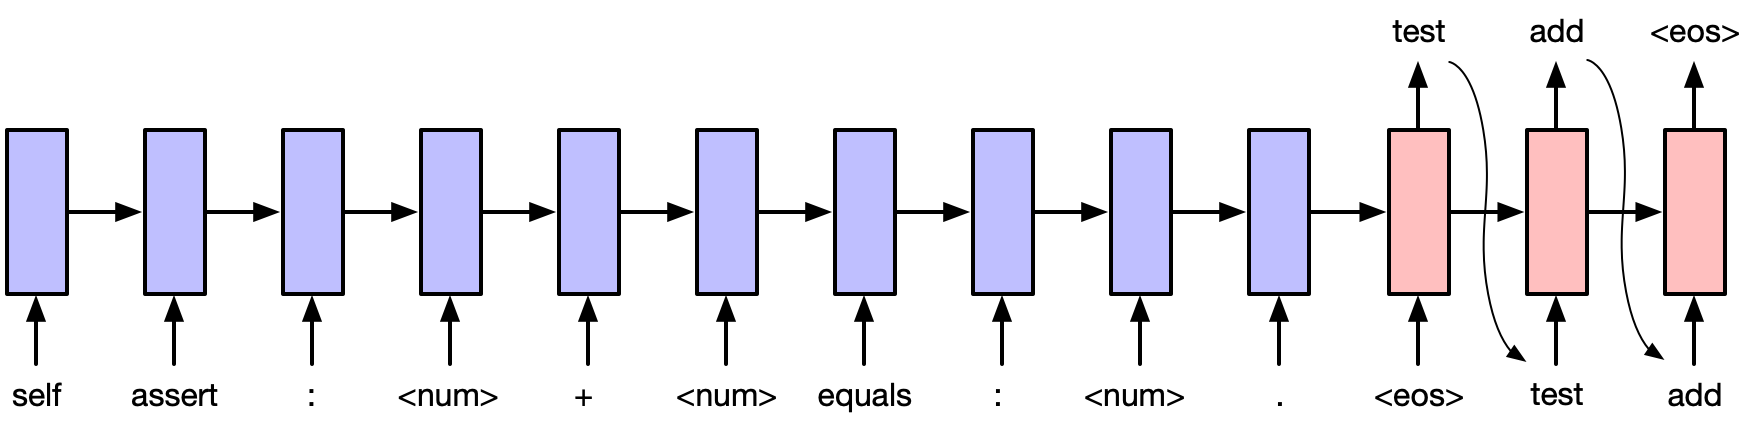
\includegraphics[width=\columnwidth]{seq2seq}
\end{figure}

Attention mechanism ensures that extent to which a certain token of the input sequence $x_k$ affects the output does not depend on its position $k$. This was especially important in our case. On average English, sentences have around 20 words. But the average number of source tokens in methods from our dataset exceeds 130. By using attention we can be sure that by the time the information from first tokens reaches the decoder, it will not be saturated. Regardless of its position in the input sequence, every token has the same chance to affect the decision and the only decoder decides to which tokens it wants to pay more attention.

We used GRU cells to avoid exploding and vanishing gradient and chose them over LSTM because they have fewer parameters to train and allow us to learn faster. Because of the big length of input sequences that we feed to our network we chose the hidden vector of size 256, which is larger than what is typically used for machine translation with the sequence to sequence networks.

\section{First look at the results}
\label{sec:TranslatingCode-Results}

In this section, we do a manual overview of the method names proposed by our model. Different approaches to the numeric evaluation of these results are discussed in Chapter \ref{chap:Evaluation}. All methods presented in this section are taken from the test set. The model has not seen any of them during training.

% , briefly discuss their validity and explore the attention to see the connection between certain source tokens and the generated names.

\begin{lstlisting}
"Real name:       test is comment
 Generated name:  test is comment"
self assert: self newNode isComment.
\end{lstlisting}

\begin{lstlisting}
"Real name:       color
 Generated name:  color"
r := aColor red.
g := aColor green.
b := aColor blue.
a := aColor alpha.
\end{lstlisting}

\begin{lstlisting}
"Real name:       accept with
 Generated name:  accept"
aVisitor
  visitDraggableInteractreion: self
  with: args.
\end{lstlisting}

\begin{lstlisting}
"Real name:       add package
 Generated name:  add package"
aPackage isPackage ifFalse: [^self].
self
  addElement: aPackage
  in: self packages.
\end{lstlisting}
%
% {\lstset{basicstyle=\footnotesize}
% \begin{table}[H]
%   \begin{tabular}{|L{7cm}|l|l|}
%     \hline
%     Source code &
%     Proposed name &
%     Real name \\
%     \hline
% \begin{lstlisting}
% self assert: self newNode isComment.
% \end{lstlisting} &
%     test is comment &
%     test is comment \\
%     \hline
% \begin{lstlisting}
% r := aColor red.
% g := aColor green.
% b := aColor blue.
% a := aColor alpha.
% \end{lstlisting} &
%     color &
%     color \\
%     \hline
% \begin{lstlisting}
% aVisitor
%   visitDraggableInteractreion: self
%   with: args.
% \end{lstlisting} &
%     accept &
%     accept with \\
%     \hline
% \begin{lstlisting}
% aPackage isPackage
%   ifFalse: [^self].
% self
%   addElement: aPackage
%   in: self packages.
% \end{lstlisting} &
%     add package &
%     add package \\
%     \hline
%   \end{tabular}
% \end{table}}
